\documentclass[11pt]{amsart}
\usepackage{geometry}                % See geometry.pdf to learn the layout options. There are lots.
\geometry{letterpaper}                   % ... or a4paper or a5paper or ... 
%\geometry{landscape}                % Activate for for rotated page geometry
%\usepackage[parfill]{parskip}    % Activate to begin paragraphs with an empty line rather than an indent
\usepackage{graphicx}
\usepackage{amssymb}
\usepackage{epstopdf}
\usepackage{hyperref}
\usepackage{graphicx}
\usepackage{subfigure}


\theoremstyle{mydef}
\newtheorem{definition}{Definition}
\newtheorem{conj}{Conjecture}[section]


\DeclareGraphicsRule{.tif}{png}{.png}{`convert #1 `dirname #1`/`basename #1 .tif`.png}

\title{On (mod N) Spirals}
\author{Andrew Reiter\\
arr@watson.org}
%\date{}                                           % Activate to display a given date or no date

\begin{document}
\maketitle
\section{Introduction}
This note is intended to introduce the process of constructing (mod N) spirals and the idea of a \textit{complete spiral}.  It also introduces a few conjectures related to patterns seen in the construction of \textit{complete spirals}; regarding the lengths of sides, iteration counts, and ending corners of these objects. While not inspired by Ulam's Spiral, the construction of  a (mod N) spiral quite is similar to it's construction, although I proceed clockwise. I am unaware of other work or literature on this topic, so have no references other the couple related to code. I realize the vastness of this field's literature base, so it is clear that I likely have missed something; in part this is why I wrote it up. Further, I found the investigation a lovely pursuit, so if that is all that comes of this work, then I am happy.

\section{Spiral Construction}
Here I describe the construction of a (mod N) spiral and much of the notation defined and assumptions made here are used with same notion after this section.

Let $N \in \mathbb{Z}$ and $N \ge 2$. Let $S_N = \{ 0, 1, ..., N-1 \}$. Let $L$ be a square lattice. 

Choose a point $l_0 \in L$ and it will be the starting point of the spiral; choose $l_0 = (0, 0)$, the origin. Let $l^*_0$ be the value assigned to the point $l_0$. We want to assign the first element of $S_N$ to the first point in the spiral, thus, we assign $l^*_0 = 0$. Now, we wish to choose a second point in the spiral, $l_1$, by moving in the positive $x$ direction by one unit and assign it the second value of $S_N$. So we have $l_1 = (1, 0)$ and $l^*_1 = 1$.  We will continue to choose points $l_i$ and assigning values from $S_N$ in an increasing order.

\begin{figure}[h]
\centering
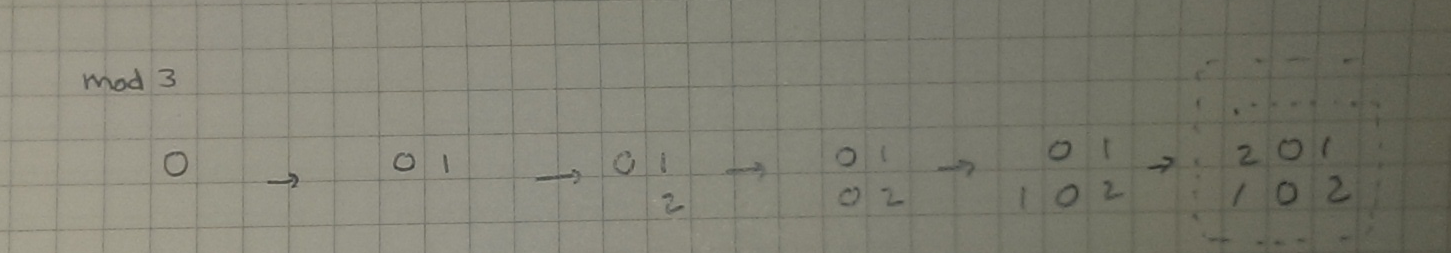
\includegraphics[scale=0.3]{mod3basic.png}
\caption{Building a (mod 3) spiral}
\label{fig:mod3spiral}
\end{figure}

To continue this process, let us try to visualize us being on the lattice work itself. Orient your mind so that previous move to $l_1$ was you ``moving forward''. With current position $l_1$, check the lattice point to your right: if it is assigned a value already, move ``forward'' to the next lattice point. However, if the lattice point to the right was \emph{not} occupied, then you ``turn right'' and ``move forward'' to occupy it. You are now at $l_2$ and have $l^*_2 = 2$ and, based on above, $l_2 = (1, -1)$. . You repeat this pattern of ``looking right'' to determine if you should ``turn right'' or keep ``moving forward'' and then assigning values from $S_N$. Continuing on with the lattice points we find $\{ l_i \}^{6}_{i=3} = \{  (0, -1), (-1, -1), (-1, 0), (-1, 1) \}$

At some point, the process will reach a lattice point $l_i$ in which $l^*_{i-1} = N-1$. This is means an \textit{iteration of (mod N)} has occurred and we assign $l^*_i = 0$. This restarts going through values of $S_N$. The (mod N) spiral is the set of tuples $\{ (l_0, l^*_0), (l_1, l^*_1), ... \}$ 





\begin{figure}[h]
\centering
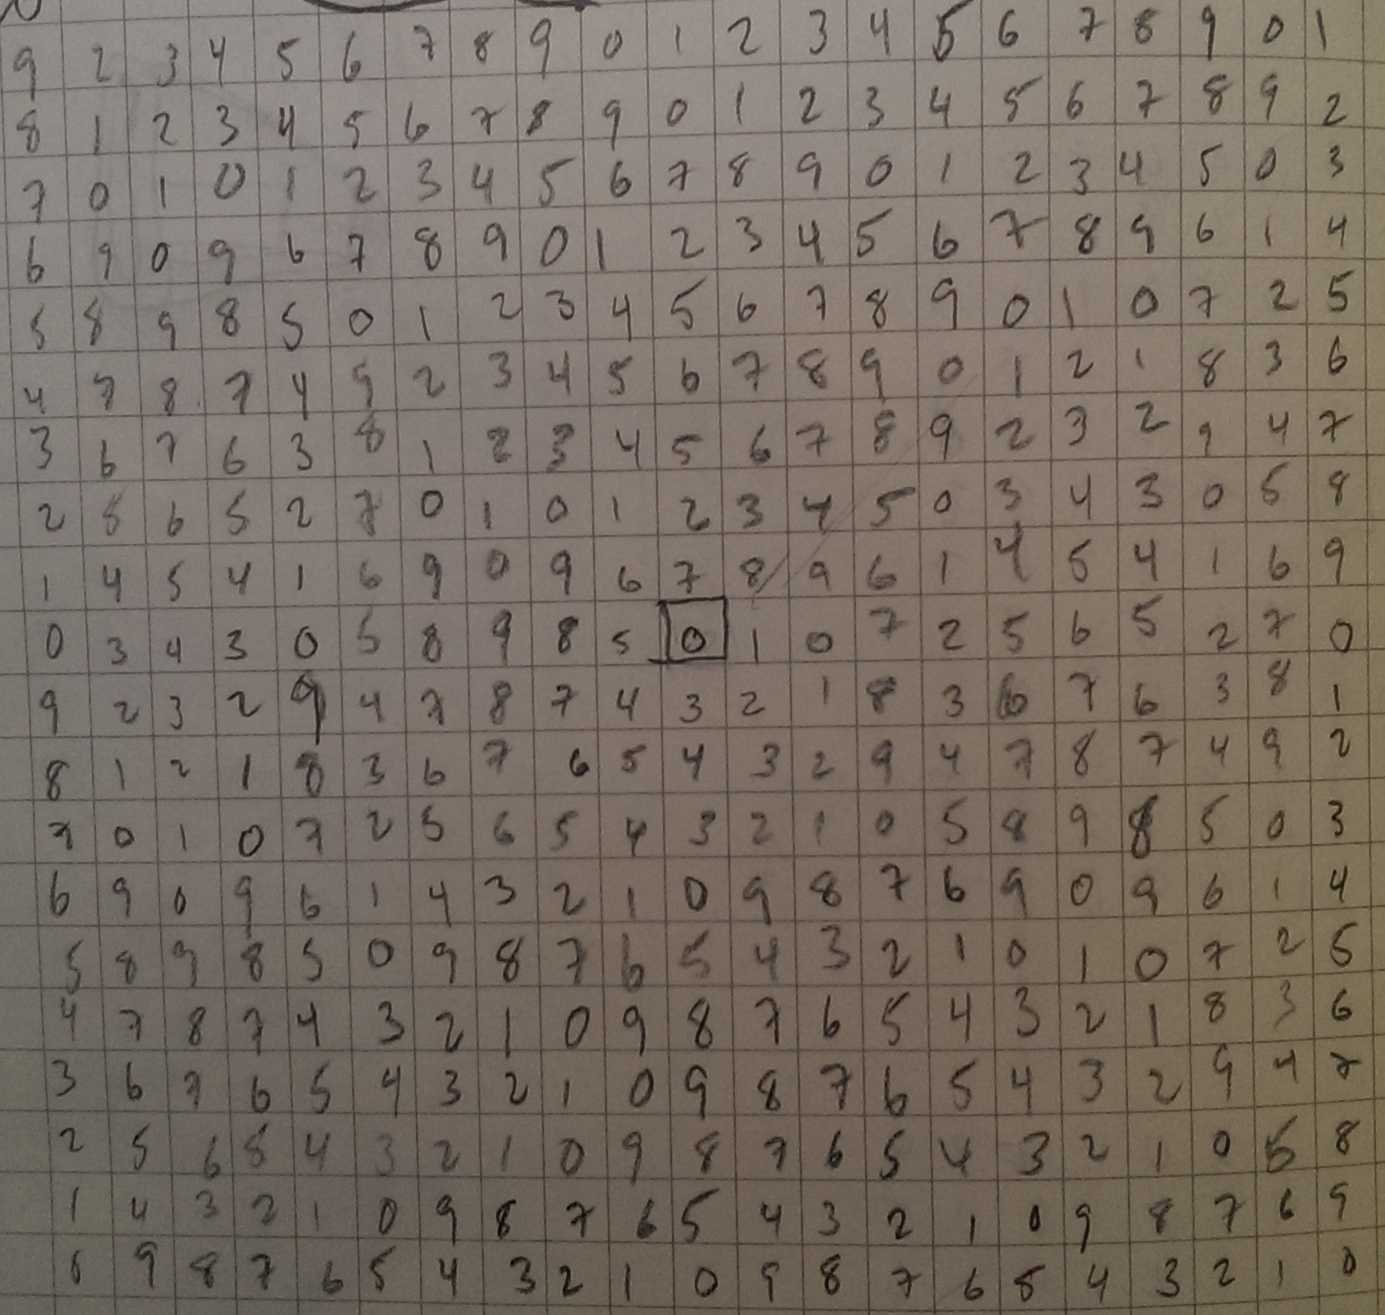
\includegraphics[scale=0.3]{mod10.png}
\caption{a (mod 10) spiral}
\label{fig:mod10}
\end{figure}

The purpose of inventing notation for the lattice points is to help give a scalar mapping into the lattice based on the spiral. Currently, I do not use it, but I imagine it could be used in describing some diagonal patterns seen in figure \ref{fig:mod10}; this is the construction of a (mod 10) spiral. The starting location, $l_0,\ l^*_0 = 0$, is marked by a box.



\section{complete spiral}
My initial interest in generating spirals of increasing size for various (mod N) was to see more of the diagonal patterns as referred to above and seen in figure \ref{fig:mod10}. In thinking about how to do this in strict manner, I created the following definitions.

\begin{definition}[complete spiral]
A complete spiral is achieved when in the spiral construction you reach a point where $l^*_i = N-1$, $l_i$ is on a corner, and the lengths of the outermost sides are equal.
\end{definition}

\begin{definition}[k-th square of (mod N)]
The first complete spiral reached in the spiraling process is k=1, or 1-st square of (mod N),  $Sp^1_N$. Iterating further and reaching other complete spirals, we increment $k$ and have $Sp^k_N$.
\end{definition}

These two definitions also prompted me to think about how many times one goes through $S_N$ in creating a complete spiral; thus the following definition.

\begin{definition}[Iterations of $Sp^k_N$]
The number of times $S_N$ is used in order to reach the k-th square is the iteration count.
\end{definition}

\begin{figure}[h]
\centering
\subfigure{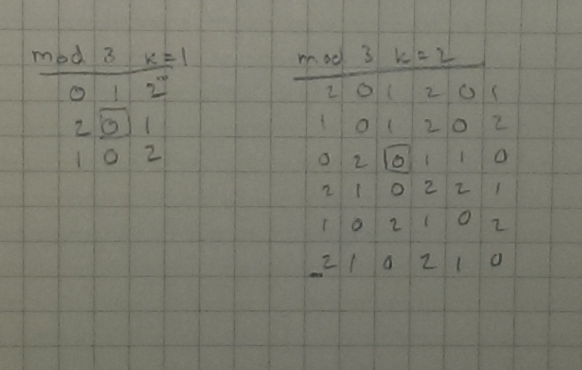
\includegraphics[height=4cm]{mod3k12.png}}
\subfigure{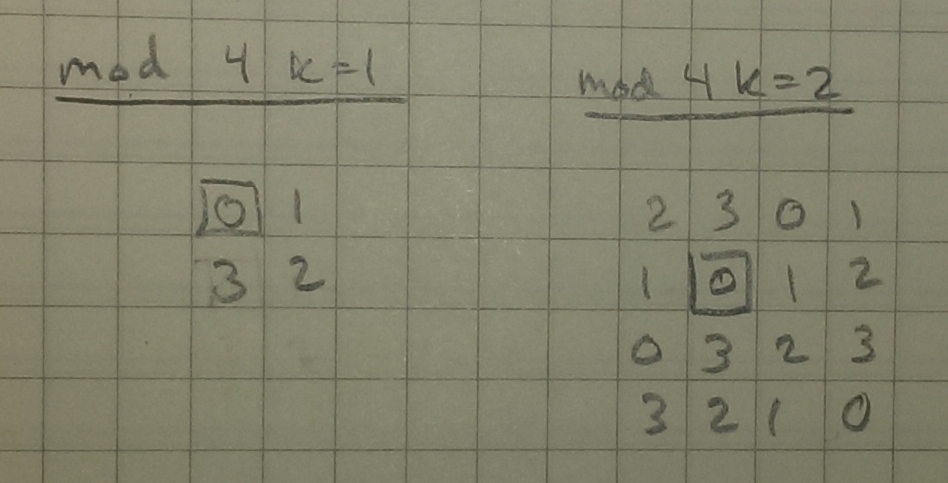
\includegraphics[height=4cm]{mod4.png}}
\caption{$Sp^1_3$ and $Sp^2_3$ on the left, $Sp^1_4$ and $Sp^2_4$ on the right}
\label{fig:mod34}
\end{figure}

We see in figure \ref{fig:mod34} the cases of (mod 3) for $k=1,2$.  In the case of $Sp^1_3$, it is a 3-by-3 square and took 3 iterations of $S_3$. For $Sp^2_3$, it results in 6-by-6 and 12 iterations. With $Sp^1_4$, we see 2 and 1, and $Sp^2_4$, we see 4 and 4.

I pursued generating spirals with pencil and paper in a manner by which I would create sets of complete spirals for various (mod N). While tedious and not exactly related to my initial goal of looking at diagonal patterns, it helped me to realize there seemed to be patterns found in the construction of the spirals. Specifically in the sizes of the complete spirals, iteration counts, and where the last lattice point rested; this led me to investigate what the patterns were.

\subsection{On the side lengths and iterate counts of $Sp^k_N$}
In order to investigate these patterns, I determined that more data was needed and, due to the tedium of pencil and paper, a program should be written to generate complete spirals \cite{PySquare}. This allowed me to generate a larger number of complete spirals and collect data on lengths, iterations, and ending points. 

In looking at the initial data, for small $N, k$, I easily saw a few common patterns in tuples of (lengths, iterations) including $(kN, k^2N)$, $(\frac{kN}{2}, \frac{k^2N}{4})$, and $(\sqrt{N}k, k^2)$. However, these were not working for all values and not discernible pattern for how to choose which mapping to use for given $N, k$. After some thinking and continual looking at the data generated from \cite{PySquare}, I realized there was some relation to the prime factorization of $N$ that would determine the lengths and iterations. I modified the program to print the prime factorization of $N$ for each complete spiral $Sp^k_N$, along with the lengths and iteration data. From this information I realized that there was something related to squares of primes of the factorization of $N$; this led me to realize the two conjectures below on lengths and iterations. Before the conjectures, I will describe the process of finding maximum perfect squares in a factorization of a positive integer, which seems to be the link to determining $Sp^k_N$ lengths and iteration counts.


\subsubsection{Finding Maximal Perfect Squares in Factorizations}

By demonstrating the process of determining a set of \textit{maximal perfect squares of a factorization of N}, I hope to illustrate what they are.

Let $P_N = \{p_i\}$ be the prime factorization of a positive integer $N$. Let us augment $P_N$ by including $\{1, 1\}$ as factors, so $P^*_N = \{1, 1\} \cup P_N$.

Let $P^p_N$ be the partitioning of $P^*_N$ by value of $p_i \in P^*_N$. That is, $P^p_N = \{ \{ 1, 1 \}, \{ p_j \}_j, \{ p_k \}_k, \ldots \}$ so each element of $P^p_N$ is a set that contains all of the prime factors of $N$ of the same value. 

Define a set $R_N = \{ \}$ that will hold the maximum perfect squares of $N$. 

Iterate through $\rho \in P^p_N$. If $\left\vert \rho \right\vert < 2$, then move onto the next element in $P^p_N$. However, if $\left\vert \rho \right\vert \ge 2$, attempt to determine the maximum perfect square found when taking the product of the elements in $\rho$. Start by letting $s = \prod\limits_i \rho_i$. If $s$ is a perfect square, then $R_N = R_N \cup \{ s \}$ and iterate onto the next $\rho \in P^p_N$. If $s$ is not a perfect square, then set $s = \frac{s}{\rho_i}$ and test for perfect squareness again, ... until you minimally reach $\rho^2_i$. At this point, set $R_N = R_N \cup \{ \rho^2_i \}$, and then iterate onto the next  $\rho \in P^p_N$.

The resultant set, $R_N$, is the set of maximum perfect squares of $N$. Note that if $N$ is \textit{squarefree} that $R_N = \{ 1 \}$. 

As an example let $N=8$, so we have $P^p_8 = \{ \rho_1, \rho_2 \} = \{ \{1,1\}, \{2, 2, 2\} \}$. Iterating through $\rho \in P^p_N$, we first see $\{1,1\}$ and thus add $1^2$ to $R_8$. Next, we have $\rho_2 = \{ 2, 2, 2 \}$. Set $s = \prod\limits_3 2 = 8$. It is not a perfect square. Let $s = \frac{s}{2} = 4$. Since $4$ is a perfect square we add it to $R_8$. Since there are no more elements of $P^p_8$ to iterate through, the maximum perfect squares of $N$ are $R_8 = \{ 1, 4 \}$.

For another example, have $N=216$ leads to $P^p_{216} = \{ \{1,1\}, \{2, 2, 2 \}, \{3, 3, 3\} \}$. We know what happens with 1 and 2, but for 3, $s = \prod\limits_3 3=27$ which is not a perfect square, so must use $\frac{s}{3}=9$. Thus, we have $R_{216} = \{ 1, 4, 9 \}$

And for $N=256$, we have $P^p_{256} = \{ \{1,1\}, \{2, 2, 2, 2, 2, 2, 2, 2\} \}$. This means $s = \prod\limits_8 2 = 256$ which is perfect square, so $R_{256} = \{ 1, 256 \}$. In this case, you can see that there are multiple perfect squares found by taking product of 2 in different counts, but we are looking for the maximal square.

For yet another case $N=255$ where $N$ is \textit{squarefree}, $P^p_{255} = \{ \{1,1\}, \{ 3 \}, \{ 5\}, \{17\} \}$. Only 1-collection has cardinality of greater than 1. Thus, $R_{255} = \{ 1 \}$.

I am uncertain as to keeping the squared value in $R_N$ versus  storing the root; currently, I view things from the squared value perspective.


\begin{conj}[Length of Sides of $Sp^k_N$]
Let $\lambda$ be the length of the sides of $Sp^k_N$. If $\{R_i\}$ be the set of maximal perfect squares in the factorization of $N$, then, $\lambda = \frac{kN}{\prod\limits_i \sqrt{R_i}}$.
\end{conj}

\begin{conj}[Iteration Count of $Sp^k_N$]
Let $\xi$ be the iteration count  of $Sp^k_N$. If $\{R_i\}$ be the set of maximal perfect squares in the factorization of $N$, then, $\xi = \frac{k^2N}{\prod\limits_i R_i}$.
\end{conj}

One can clearly see the relation between $\lambda$ and $\xi$. 

One will note that in the case where $N$ is a product of just one of each prime factor, the formulae reduce to $\lambda = kN$ and $\xi = k^2N$. These can also be considered an upper bound. It is interesting to me that in these cases, $N$ is a \textit{squarefree} integer and have the least robust length and iteration count mappings.

\subsection{Ending Corner of $Sp^k_N$}

Another pattern in the generation of \textit{complete spirals} that was noticed is related to which corner the last lattice point comes to rest. It seems to end on either the top right or bottom left corner and this depends on values of $N$ and $k$. One can see this in figure \ref{fig:mod34}.

\begin{conj}[Ending Corner]
If $l_{max} \in L$ is the last lattice point in the complete spiral $Sp^k_N$, then $l_{max}$ is either the top-right corner or bottom-left corner. If $N$ even, then $l_{max}$ will always be the bottom-left corner. If $N$ odd and $k$ odd, then $l_{max}$ will be the top-right corner of $Sp^k_N$. If $N$ odd and $k$ even, then $l_{max}$ will be the bottom-left corner.
\end{conj}

\subsection{Cases Verified}
I have verified the conjectures on length, iteration count, and end corners for $N=2\ldots350$ and $k=1\ldots5$. This code may be found at \cite{PySquare}. At this location, if you view the file \textit{run.log} you will see log output of the code running.

\subsection{Grayscale Visualization}

In the process of investigating sizes and iteration counts of $Sp^k_N$, I implemented a method to map the generated spirals to grayscale images. This works best for positive integers, $N$, less than 256. I define the map as $f : \{ 0, 1, \ldots, N-1 \} \mapsto \{ 0, floor(\frac{255}{N}), 2floor(\frac{255}{N}), \ldots, (N-1)floor(\frac{255}{N}) \}$. The mapping $f$ takes $S_N$ to a set of brightness values. These brightness values are easily used to create grayscale images.

An example of this is $Sp^{29}_{28}$ seen in figure \ref{fig:viz2928} and $Sp^{30}_{16}$ seen in figure \ref{fig:viz1630}.

\begin{figure}[h]
\centering
\includegraphics[scale=0.7]{N28k29a.png}
\caption{grayscale visualization of $Sp^{29}_{28}$}
\label{fig:viz2928}
\end{figure}

\begin{figure}
\centering
\includegraphics[scale=1]{spN16k30.png}
\caption{grayscale visualization of $Sp^{30}_{16}$}
\label{fig:viz1630}
\end{figure}

However, due to computation time taking to generate the spirals and the images, I only generated $N=2...30$ for $k=1...50$. They may be viewed at \cite{GraySquare}.

\section{Conclusion}
This note has introduced (mod N) spiral construction and the idea of \textit{complete spirals} with respect to (mod N) spirals. This note also proposes a conjecture as to predicting the side lengths and iteration counts of complete spirals, $Sp^k_N$. Also introduced is a grayscale visualization of these spirals. While not introduced, there is also the I am curious as to any existing literature on this or similar work.

\subsection{Future Work}
While further verification of the conjectures is nice, ideally proofs for them would be more satisfying.
It would be of interest to think about looking at how this might work for cubes or higher dimensional squares, since the lattice is the basis for the spiral. Further, it might be interesting to see how one might spiral with objects in $\mathbb{R}^2$ such as a triangle.
\subsection{Acknowledgments}
Recognizing Veracode Research for providing time to think about this, Jared Carlson of Veracode Research, and Prof. Rob Kusner of UMASS-Amherst.

\begin{thebibliography}{1}
\bibitem{PySquare} A. Reiter, \url{https://github.com/cwcomplex/modNspirals}
\bibitem{GraySquare} A. Reiter, \url{https://github.com/cwcomplex/modNspirals/tree/master/somegrey}

\end{thebibliography}



\end{document}  